\documentclass[a4paper, 12pt]{article}

\usepackage[T1]{fontenc}
\usepackage{IEEEtrantools}
\usepackage[]{amsmath}
\usepackage{amssymb}
\usepackage{float}
\usepackage[]{graphicx}
\usepackage{subfig}
\usepackage{caption}

\title{Control Systems: Practical 4}
\author{Ruan de Bruyn \and 216054484 \and Quintin Kruger \and 216008466}

\begin{document}

\pagenumbering{gobble}
\maketitle
\newpage
\pagenumbering{roman}
\tableofcontents
\listoffigures
\newpage
\pagenumbering{arabic}

\section{Introduction} % (fold)
\label{sec:introduction}
The purpose of this practical is to model discrete controllers using approximation methods to convert a continuous controller to a digital controller  and a more accurate approach where a complete digital design of the plant and controller is done. Used in this practical is a lead compensator defined by the equation that follows
\begin{equation}
	\label{eq:lead_compensator}
	D_c(s) = 
\end{equation}

<+DISCUSSION OF THE PLANT+>
% section introduction (end)

\section{Question 1} % (fold)
\label{sec:question_1}
The Tustin method of approximating the lead controller as defined by \eqref{eq:lead_compensator} was used to yield the discrete controller for the system in consideration. To follow are different discrete controller results obtained for a number of different sampling times 




% section question_1 (end)

\section{Question 2}

\begin{figure}[H]
	\centering
	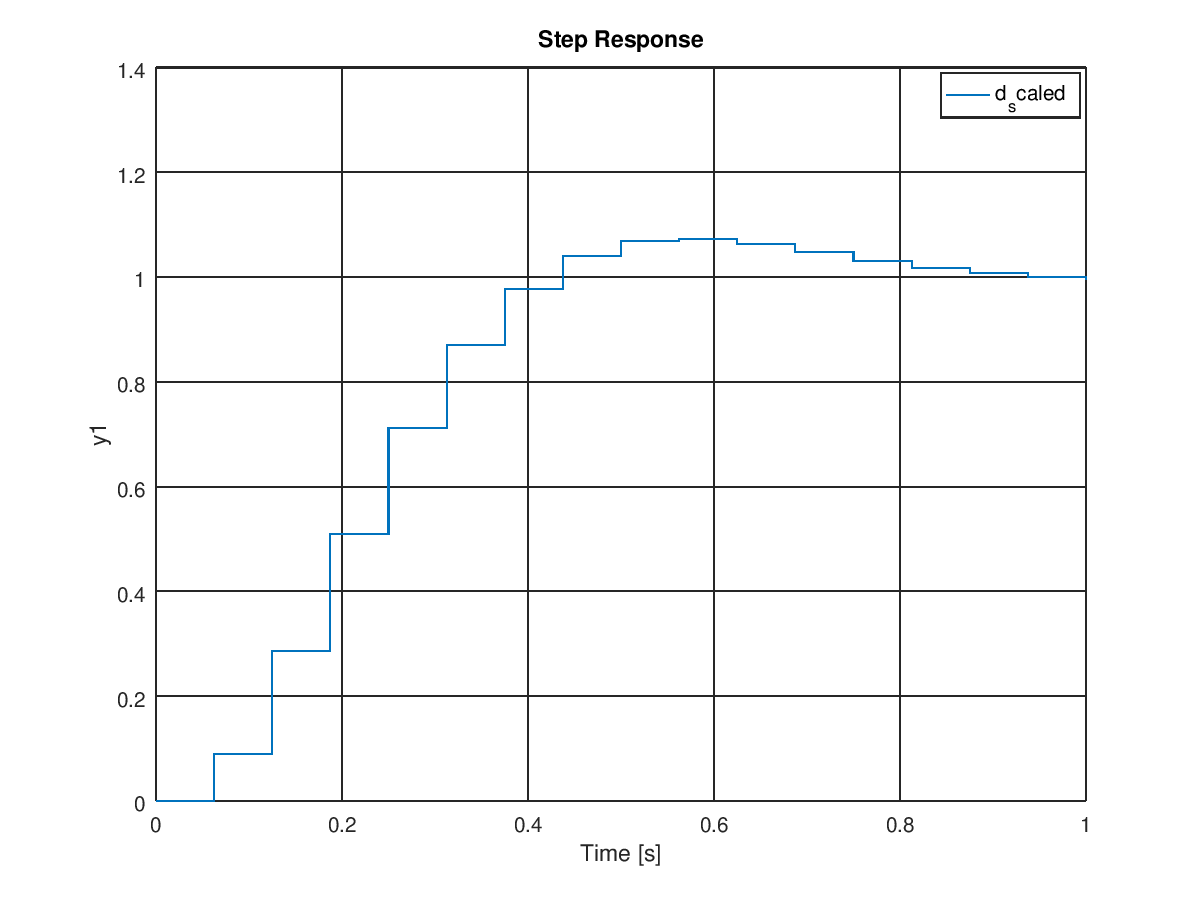
\includegraphics{./img/2_1.png}
	\caption{ZOH system}
	\label{fig:2_1}
\end{figure}

Pole locations: -5 += 6j
Sampling time = 0.6s

% section question_2 (end)
\end{document}
